Nous avons choisi de créer notre serveur sur une base de servlet. Ce fût ici
aussi un point nouveau pour nous, réiterant les phases d'analyse, de
découverte, de test et de mise en place. Le fonctionnement est basé sur les
échanges de requêtes type HTTP, où à chaque demande correspond une réponse. 

		
\subsection{JSON}
	Soucieux des performances et de la rapidité des échanges entre applications et
	serveur, nous avons mis en place un protocole de communication client/serveur
	où les messages transitant sont des flux JSON\footnote{JavaScript Object
	Notation :  format de données textuel issu du JavaScript (ECMAScript pour plus
	exact) où il était employé comme une syntaxe pour décrire les valeurs des
	instances d’objets}. 	
	Contrairement au XML qui peut représenter des données orientées document,
	JSON se focalise sur la description d’objets.
	Un autre avantage reconnu de JSON par rapport à XML est qu’il est nettement
	moins verbeux que ce dernier.
	Quoi qu’il en soit JSON reconnait la philosophie des services web exposant
	une interface d’échange : il s’agit
	d’envoyer et de recevoir des informations dans un format facilement manipulable par
	le protocole de transport HTTP.
	
	
	Voilà pourquoi le JSON semblait être un format de données d'échanges optimal
	pour véhiculer le plus d'informations avec une taille moindre. Il est aussi en
	adéquation avec notre politique d'utilisation web pour un serveur.
	De plus étant beaucoup utilisé, nos deux
	langages mettent à disposition des outils de sérialisation de leurs objets en JSON.
	
	Ci-dessous un exemple concret de notre protocole de communication JSON entre
	serveur et application cliente.
	
		
	\begin{verbatim}
		ServletInscription
			Player => Serveur
			{["username","password"]}
			
			Serveur => Player
			{"OK"} ou {"BU"}
			
		ServletConnexion 	
			Player => Serveur
			{["username","password"]}
			
			Serveur => Player
			{"OK"} ou {"BU"}
			
		ServletGameList
			Player => Serveur
			{"userKey"}
		
			Serveur => Player
			{[{"class":"Game","map":"mapName","name":"gameName",
			 "playerNumberConnected":nbConnected,"type":"gameType"},{..},{..}]}
			 
		ServletCreateGame:
			Player => Server:
				{"userKey": <userKey>, "game": {"name":<name>, "type":<type>, "map":<map>, "ennemiesNumber": <ennemiesNumber>}}
				
			Server => Player:
				{"OK"} ou {"errorType"}
			 
		ServletConnectionGame:
			Player => Server:
				{["userKey", "gameName"]}
				
			Server => Player:
				{[<1/2/3/4>, "play<true/false>", "map", "time<mm:ss>"]} 
				ou 
				{"errorType"}
				
		ServletManageGame:
			Player => Server: 
				{"userKey", "gameName", "action"}	
				
			Server => Players: (Player, bombs, blocs, score, time)
				{[
				 [ ["x", "y", "direction", "dead <true/false>"],[...] ],
				 [ ["x", "y", "type", "explode <true/false>" ], [...] ],
				 [ ["position": {"x", "y"}, "bonus": <bonus>], [..] ],
				 [1,2,3,4],
				 "time <mm:ss>"]} 
				 ou 
				{"errorType"}
			 
			 
	\end{verbatim}
		
\subsection{Servlet}
	Comme il a été dit précédement, notre serveur est accessible via des requêtes
	HTTP contactant des servlets. Ces servlets sont stockées dans un serveur
	d'application nommé Apache Tomcat. Il s'agit d'un conteneur libre de
	servlets Java 2 Enterprise Edition, mais il fait aussi office de serveur Web.
		
	Une servlet est une classe Java qui permet de créer dynamiquement des données
	au sein d'un serveur HTTP. Une servlet s'exécute dynamiquement sur le serveur
	web et permet l'extension des fonctions de ce dernier, typiquement : accès à
	des bases de données.
	
	Lors du développement nous avons eu simplement à remplacer les
	classes(diagramme partie Modélisation) représentant les tâches par des classes
	Java de type Servlet. 
	Quant à la classe Context elle est devenue ContextListener.
	Cette dernière est
	invoquée lorsque l'objet ServletContext	est crée. Sa méthode contextInitialized(ServletContextEvent event) sera
	alors appelée, permettant ainsi de définir des objets communs à toutes les
	servlets, tels qu'un accesseur à la base de données, ou le tableau qui va
	contenir les utilisateurs connectés.
		

	\subsubsection{Schéma de fonctionnement }
		
		\begin{center}
			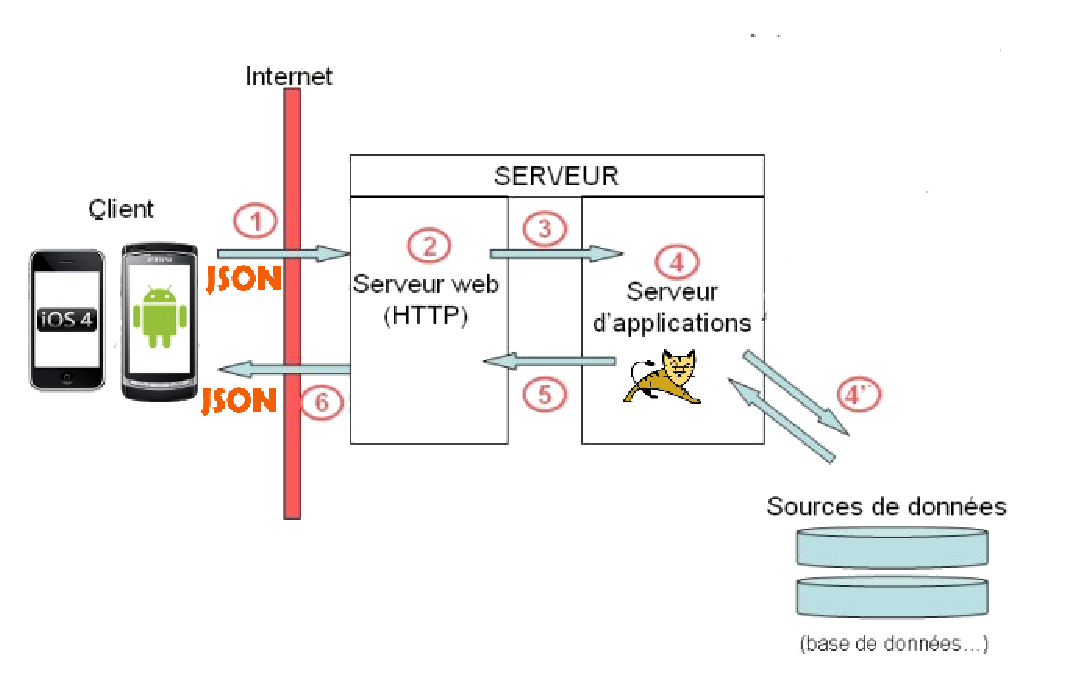
\includegraphics[width=16cm]{Analyse/Img/serveurappli.eps}
		\end{center}
		
		\begin{enumerate}

			\item 
					Le client émet une requête pour demander une
					ressource au serveur. Par exemple la création de son compte multijoueur,
					qui pourrait se situer \url{http://Bomberklob.com/inscription}
			\item
					Côté serveur, c'est le serveur web qui traite les
					requêtes HTTP entrantes. Il traite donc toutes les requêtes, qu'elles
					demandent une ressource statique ou dynamique. Seulement, un serveur HTTP
					ne sait répondre qu'aux requêtes visant des ressources statiques.

			\item 
					Ainsi, si le serveur HTTP s'aperçoit que la requête reçue est destinée
					au serveur d'applications, il la lui transmet. Les deux serveurs sont
					reliés par un canal, nommé connecteur.
		
			\item
					Le serveur d'applications (dans notre cas Tomcat) reçoit la requête à
					son tour. Lui est en mesure de la traiter. Il exécute donc la servlet
					correspondante à la requête, en fonction de l'URL, en récupérant les
					valeurs dans le flux JSON entrant. Cette opération est effectuée à partir
					de la configuration du serveur, grâce un fichier web.xml faisant le mapping
					entre URL et servlet associée.
		
					La servlet est donc invoquée, et le serveur lui fournit notamment deux
					objets Java exploitables: un représentant la requête, l'autre représentant
					la réponse. La servlet execute sa fonction et génère la réponse à la
					demande, sous forme de flux JSON. Cela peut passer par la consultation de
					sources de données, comme des bases de données (4' sur le schéma).		
		
		\end{enumerate}
		
		
	\subsubsection{En pratique}
		
		Le requetes font appel à la fonction post des servlet. Le flux entrant étant
		de type JSON, il faut déserialiser le flux dans un objet correspondant. Exemple
		l'utilisateur envoie son userName et son mot de passe crypté dans un tableau,
		sérialisé en JSON, pour pouvoir récupérer les informations nous procédons
		comme suit: 
		
		\begin{verbatim}
			BufferedReader req = 
				    new BufferedReader(new InputStreamReader(request.getInputStream()));
			OutputStreamWriter writer = 
				    new OutputStreamWriter(response.getOutputStream());
			String message = req.readLine();
			
			if (message != null) {
				  response.setContentType("text/html");
				
				   // désérialisation des infos de l'utilisateur dans une arraylist 
				  JSONDeserializer<ArrayList<String>> jsonDeserializer = 
					    new JSONDeserializer<ArrayList<String>>();
				  ArrayList<String> identifiers;
				  identifiers = jsonDeserializer.deserialize(message);
				
				  username = identifiers.get(0);
				  password = identifiers.get(1);
				  
			  ...}
		\end{verbatim}
		
		
	\subsubsection{La sécurité}
	
		Ce serveur de jeu étant hebergé sur internet et contenant des informations
		sensibles d'utilisateurs, tels que des mots de passes, il était crucial
		d'instaurer des règles de sécurité et de cryptage. 
		
		En effet lors des inscriptions ou connexion au serveur pour le mode
		multijoueur, les mots de passes sont tout d'abord cryptés côté client et
		ensuite encapsulé dans un flux JSON, pour être envoyé au serveur. Il stockera
		ainsi la chaine de caractères extraite de l'objet déserialisé. De cette
		manière à aucun moment les données confidentielles ne transiteront en clair.
		
		De plus un mécanisme semblable aux sessions est en place. Dans la
		confirmation de connexion ou d'inscription, une userKey est générée. Elle correspond en
		réalité à l'identifiant de session envoyé par le serveur. Une fois associée
		à l'username correspondant, le tout est ajoûté dans le tableau d'utilisateurs
		connectés.
		Cet userKey est ensuite nécessaire pour contacter les servlets suivantes. Si
		cet identifiant n'est pas envoyé ou n'est pas présent dans le tableaux des
		utilisateurs connectés, il sera alors impossible d'accéder aux ressources du
		serveur.
		
\subsection{BDD}

	La base de données du serveur n'est pas très complexe. En effet elle ne fait
	qu'accueillir les couples userName/password des utilisateurs dans la
	table Users. 
	Pour son accès, chaque servlet peut récupérer un objet de type Connection,
	instancié à l'initialisation du serveur. Il permettra à son tour
	de récuperer un objet de type Statement. L'application va l'employer pour
	transmettre des instructions à la base. Exemple d'insertion: 
		
	\begin{verbatim}
	Connection connection = 
	  DriverManager.getConnection("jdbc:mysql://127.0.0.1/Bomberklob", "user","user");
	Statement theStatement = connection.createStatement();
	theStatement.execute(
		     "INSERT into Users VALUES ('"+ username +"','"+password+"')");
	\end{verbatim}
	
	Bien evidemment cette adresse est remplacée par une variable, elle aussi
	présente dans le ContextListener, contenant la véritable adresse de la base de
	données.
	
	
	
	